%!TEX root = ../../main.tex


\begin{figure}[!htb]
\centering
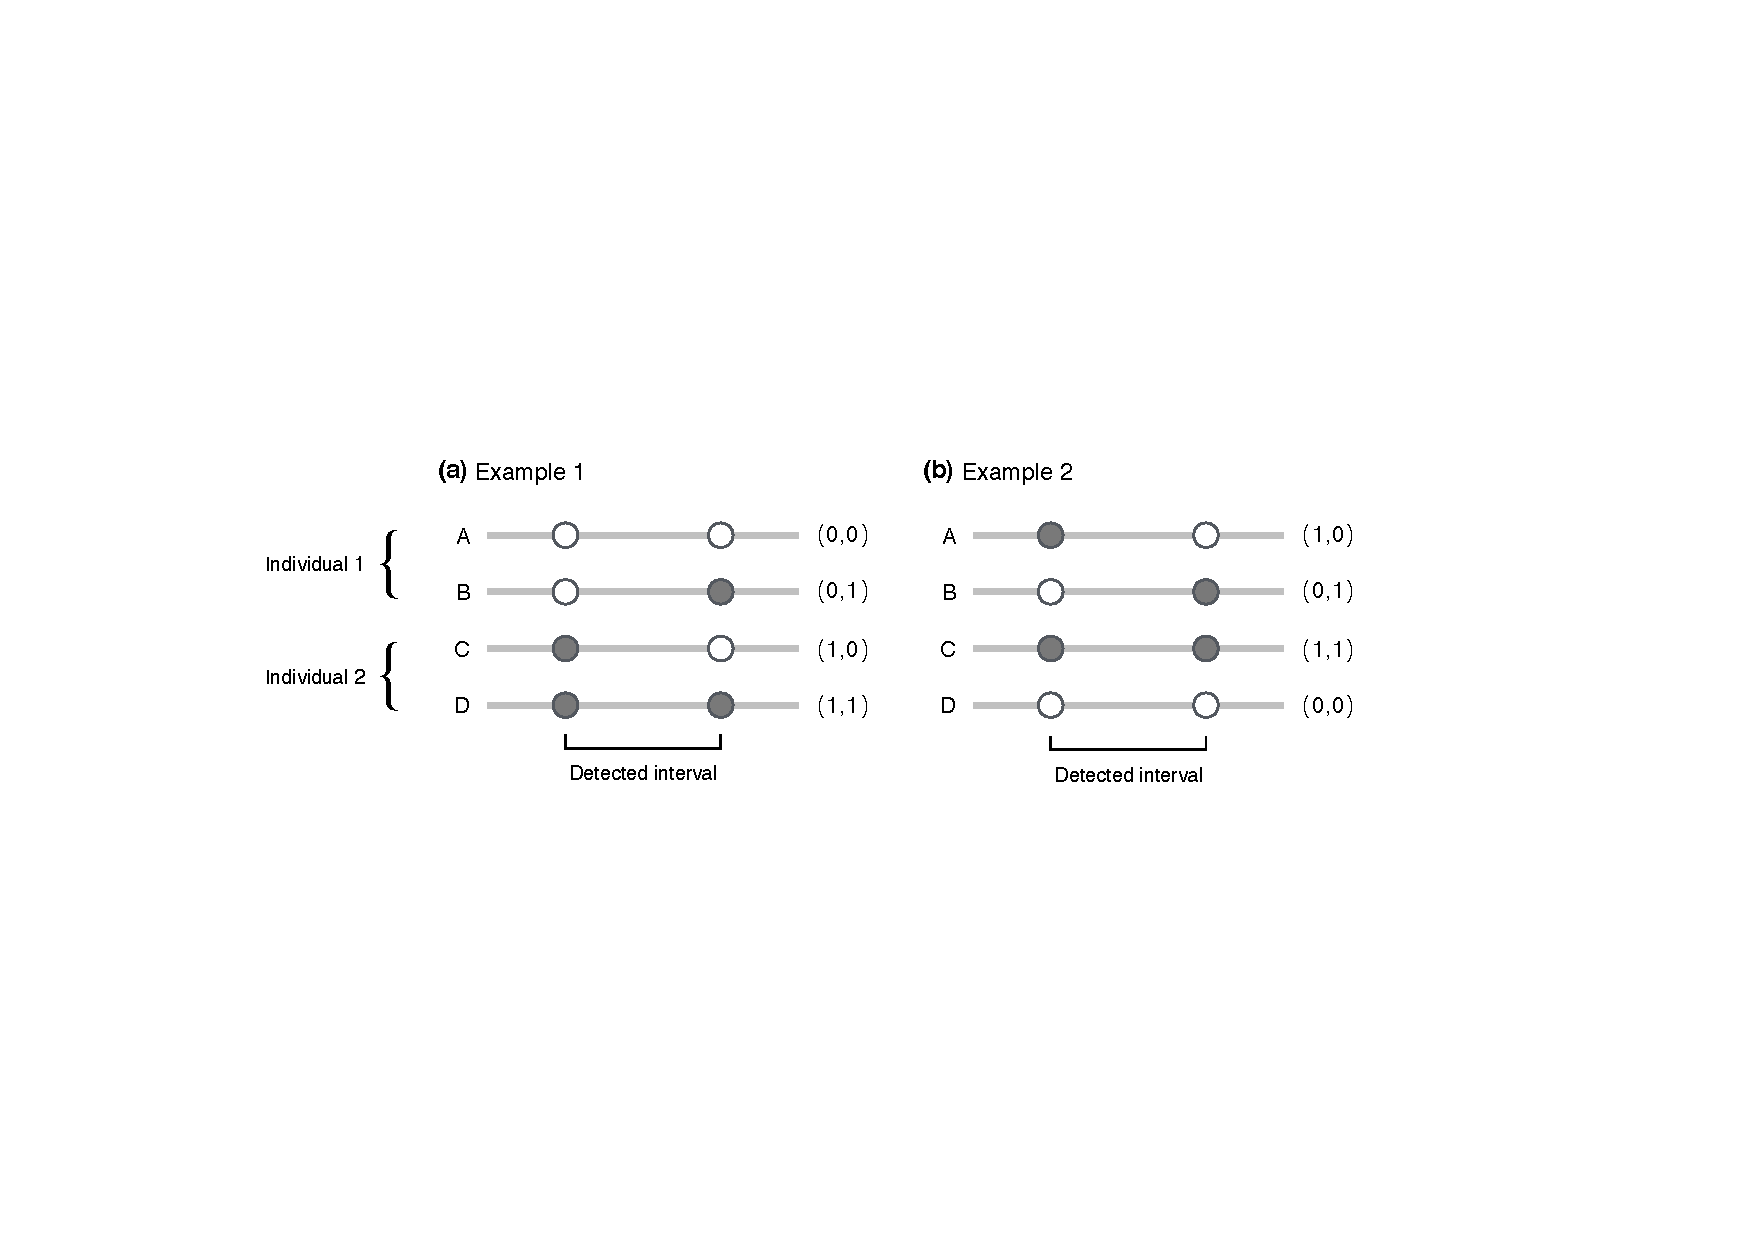
\includegraphics[width=\textwidth]{./img/ch3/info_ibdinterval}
\Caption{Example of allelic configurations satisfying the four-gamete test}
{\N{2} examples are given in which the observation of all \n{4} possible gametes is used to infer a recombination event in the history of the sample, which occurred at some location delimited by the interval spanned between the \n{2} sites.
In particular, both examples are shown with regard to the \n{2}-sample \glsentryfull{fgt}.
The \n{4} gametes (\emph{haplotypes}) are represented by horizontal lines, where ${\{A,B\}}$ belong to Individual~1 and ${\{C,D\}}$ to Individual~2.
The allelic states at the \n{2}~sites are indicated by circles and distinguish between ancestral (\emph{hollow}) and derived type (\emph{solid}).
The corresponding allelic configurations, as used in notation, are given to the \emph{right} of each gamete.
Note that all \n{4} possible gametes are found in both examples, where only their order and occurrence in individuals differ.}
{fig:info_ibdinterval}
% \vspace{-5pt}
% \hrulefill%
\end{figure}
